%%%%%%%%%%%%%%%%%%%%%%%%%%%%%%%%%%%%%%
%%%%%%%%%%%%%%%%%%%%%%%%%%%%%%%%%%%%%%
% Do not edit the TeX file your work
% will be overwritten.  Edit the RnW
% file instead.
%%%%%%%%%%%%%%%%%%%%%%%%%%%%%%%%%%%%%%
%%%%%%%%%%%%%%%%%%%%%%%%%%%%%%%%%%%%%%






\begin{knitrout}
\definecolor{shadecolor}{rgb}{0.969, 0.969, 0.969}\color{fgcolor}\begin{figure}[!h]

{\centering 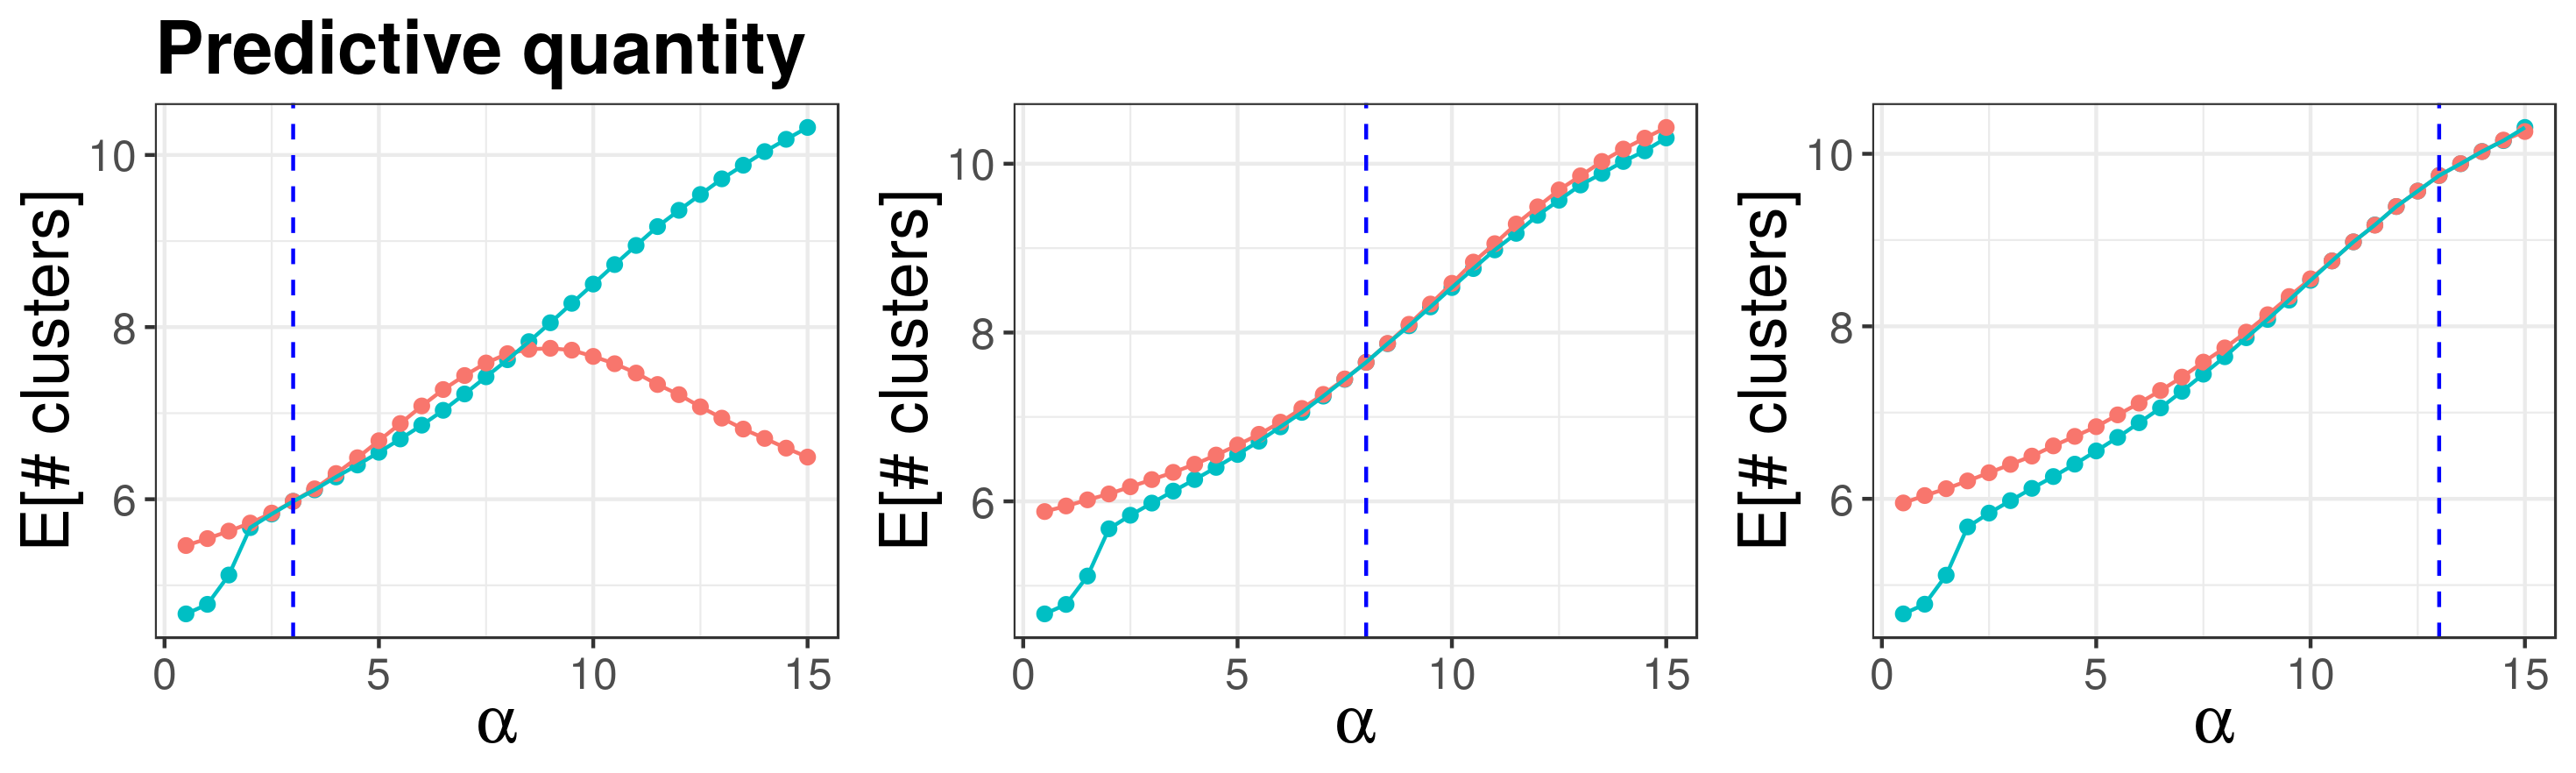
\includegraphics[width=0.98\linewidth,height=0.294\linewidth]{figure/param_sens_plot_thresh_0-1} 
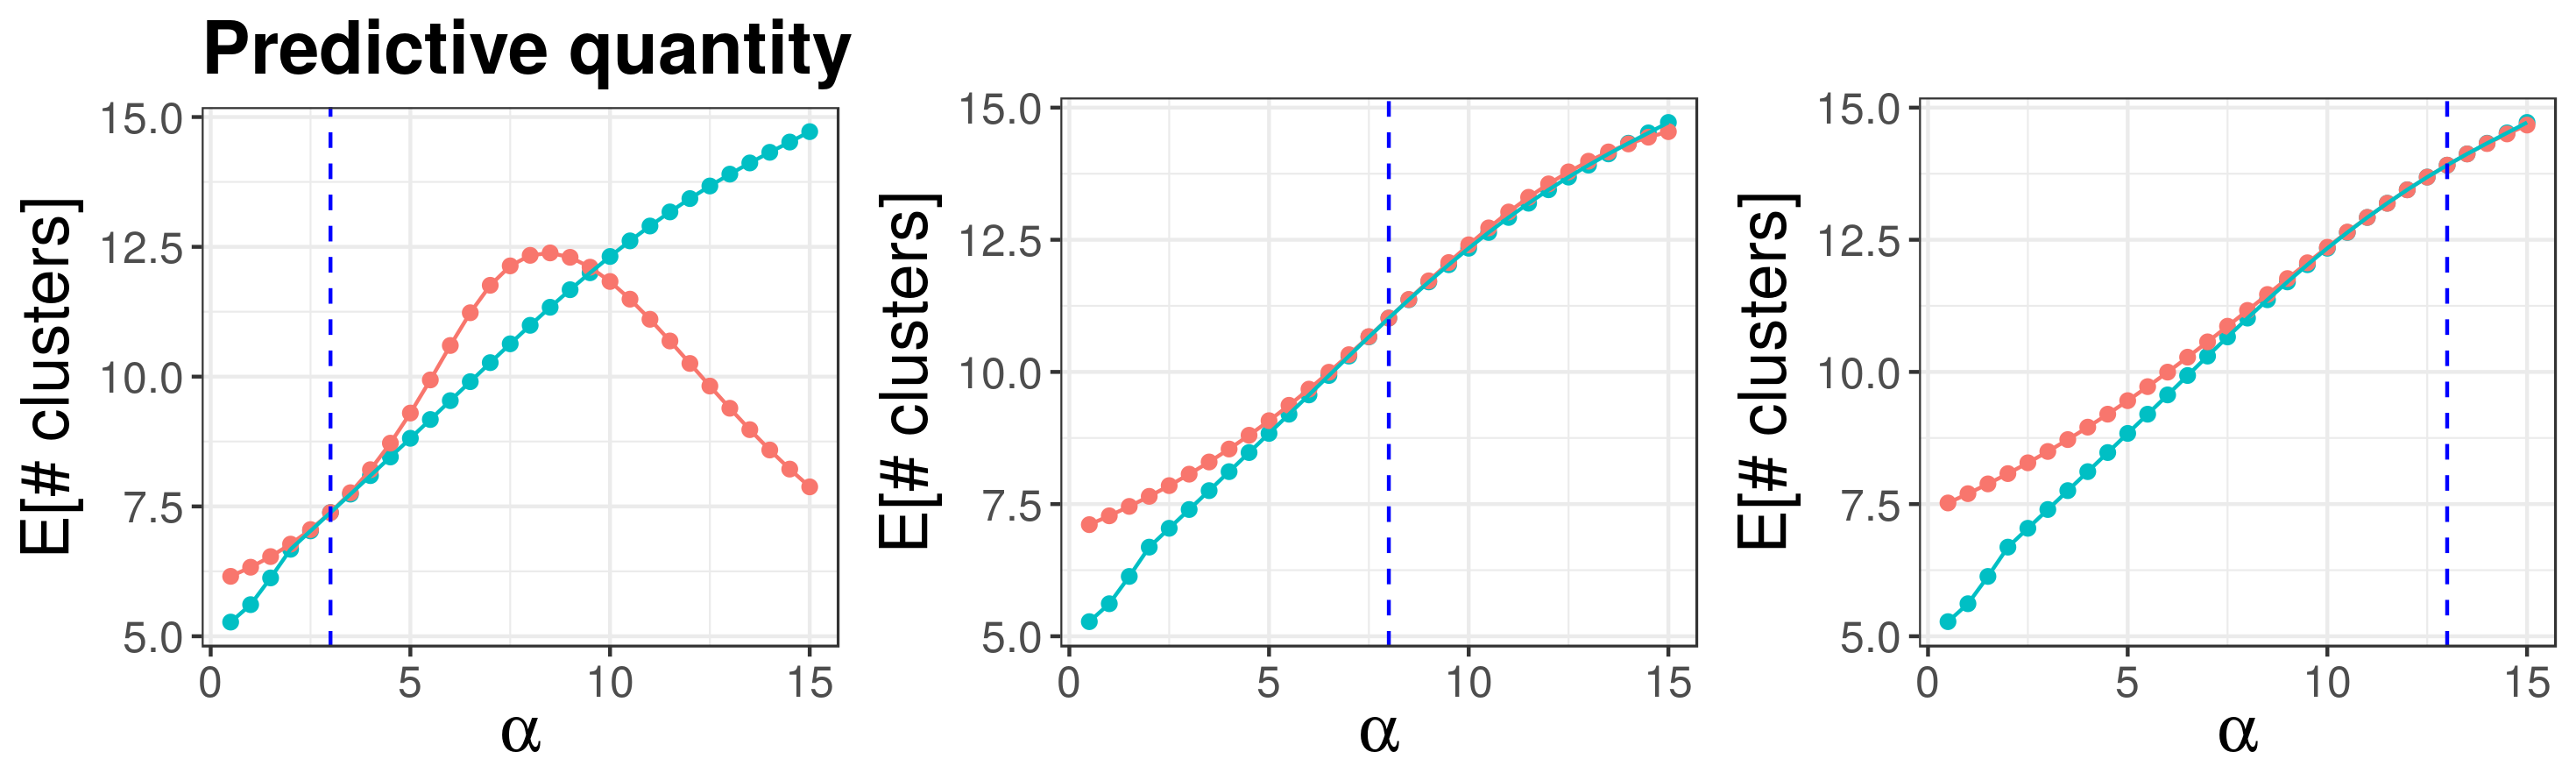
\includegraphics[width=0.98\linewidth,height=0.294\linewidth]{figure/param_sens_plot_thresh_0-2} 

}

\caption[Comparison of the expected number of clusters computed by re-optimizing versus the linear approximation]{Comparison of the expected number of clusters computed by re-optimizing versus the linear approximation.  The blue vertical line indicates the location of $\alpha_0$.Top row indicates the in-sample expected number of clusters (CITE EQUATION), while the bottom row is the preditive expected number of clusters (CITE EQUATION). }\label{fig:param_sens_plot_thresh_0}
\end{figure}


\end{knitrout}


\begin{knitrout}
\definecolor{shadecolor}{rgb}{0.969, 0.969, 0.969}\color{fgcolor}\begin{figure}[!h]

{\centering 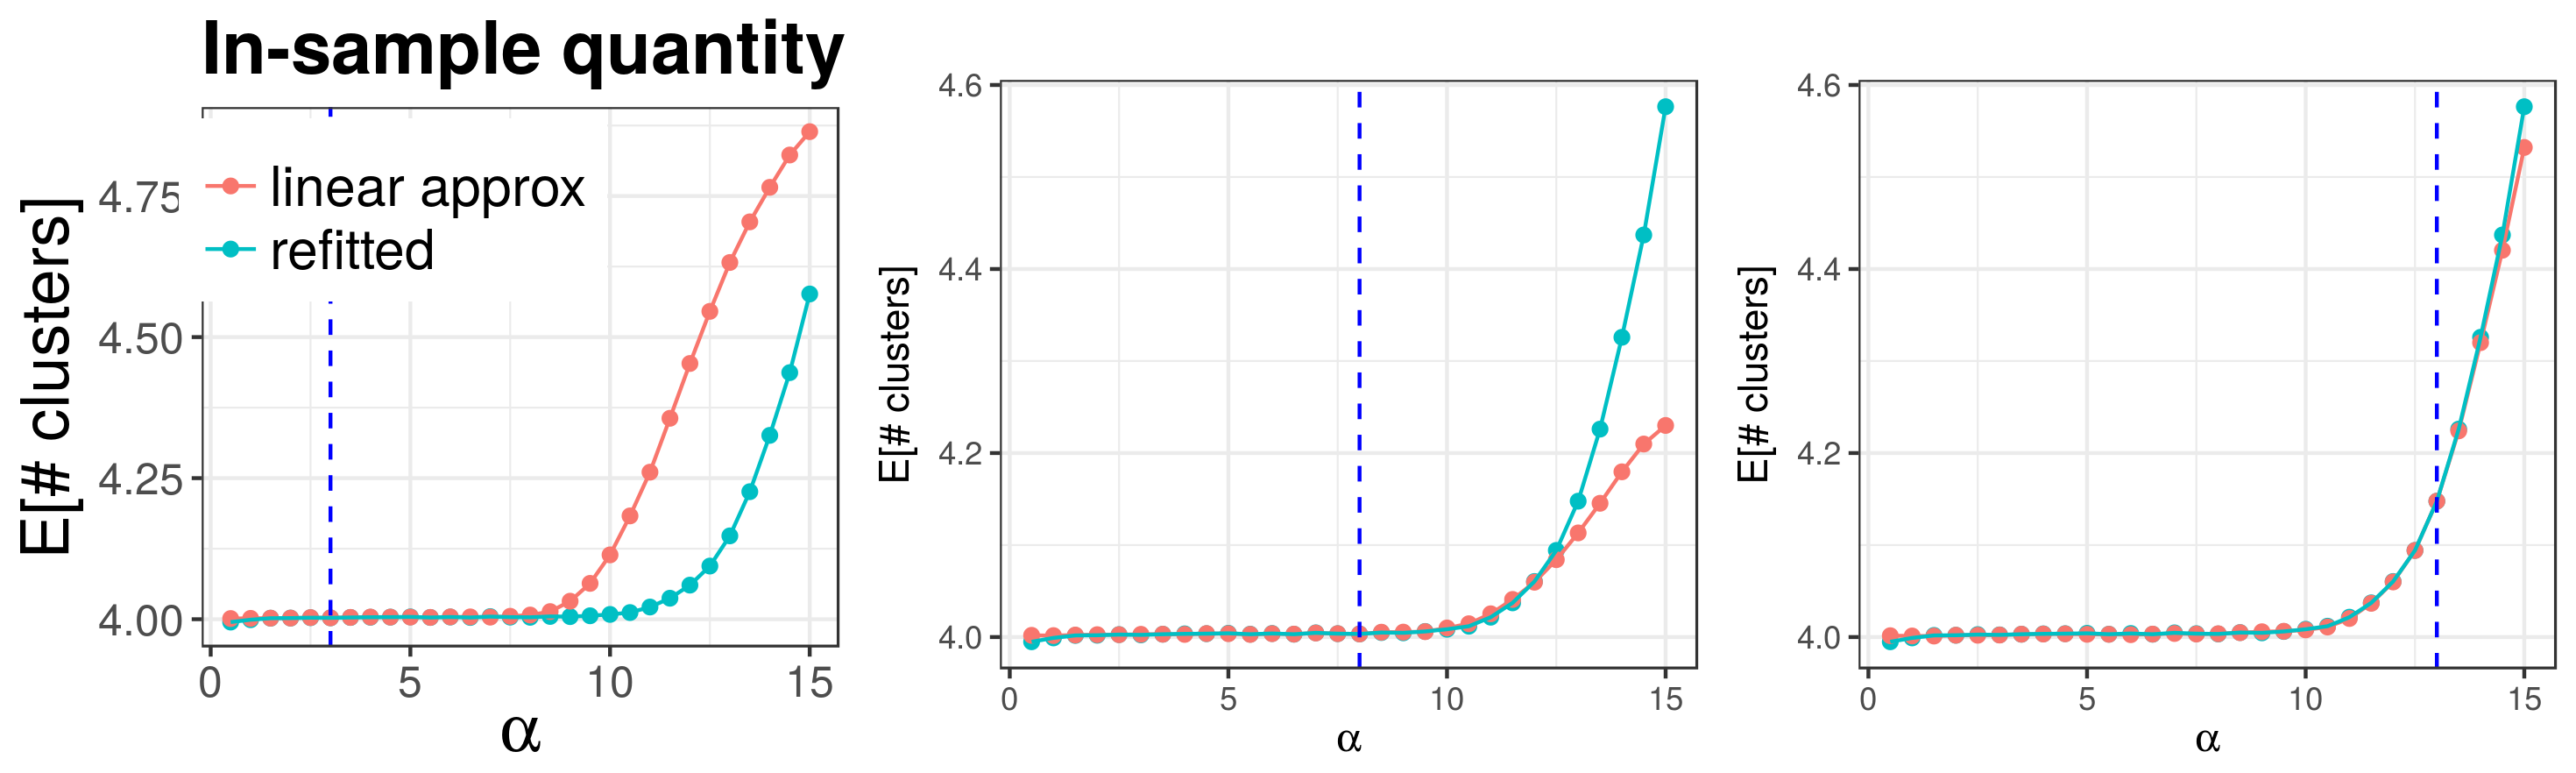
\includegraphics[width=0.98\linewidth,height=0.294\linewidth]{figure/param_sens_plot_thresh_3-1} 
\includegraphics[width=0.98\linewidth,height=0.294\linewidth]{figure/param_sens_plot_thresh_3-2} 

}

\caption[Comparison of the expected number of thresholded clusters computed by re-optimizing versus the linear approximation]{Comparison of the expected number of thresholded clusters computed by re-optimizing versus the linear approximation.  The blue vertical line indicates the location of $\alpha_0$.Top row indicates the in-sample expected number of clusters (CITE EQUATION), while the bottom row is the preditive expected number of clusters (CITE EQUATION). }\label{fig:param_sens_plot_thresh_3}
\end{figure}


\end{knitrout}
